\documentclass[a4paper]{article}

\usepackage[portuguese,english]{babel}
\usepackage[utf8]{inputenc}
\usepackage[T1]{fontenc}

\newcommand{\documentTitle}{Data Analysis and Transformation \\ TP1: Fundamentals of Signals and Systems}
\newcommand{\pdfTitle}{[ATD] TP1: Fundamentals of Signals and Systems}
\newcommand{\documentAuthors}{José Ribeiro (2008112181, jbaia@student.dei.uc.pt) \\ Pedro Magalhães (2009117002, pjrosa@student.dei.uc.pt)}

\title{\documentTitle}
\author{\documentAuthors}

\usepackage{hyperref}
\hypersetup{
	pdftitle = \pdfTitle
	,pdfauthor = \documentAuthors
	,pdfsubject = {Data Analysis and Transformation}
	,pdfkeywords = {Data Analysis and Transformation} {Signal Processing}
	,pdfborder = {0 0 0}
}

%\usepackage{subfig}
%\usepackage{amsmath}
%\usepackage{array}
\usepackage{anysize}
\usepackage{lscape}
\usepackage{amsmath}
\usepackage{graphicx}
\usepackage{caption}
\usepackage{amssymb}
%\usepackage[pdftex]{graphicx}
%\usepackage[table]{xcolor}

\hyphenation{}

\marginsize{2.7cm}{2.7cm}{3cm}{3cm}

\makeatletter

\begin{document}
\maketitle
\cleardoublepage

\tableofcontents
\cleardoublepage

\setlength{\parindent}{1cm}
\setlength{\parskip}{0.3cm}

\section{Exercise 1}
\subsection{Exercise 1.1}
\noindent Após substituição das variáveis pelo número de grupo, obtém-se a seguinte expressão:
\begin{equation}
	y[n] = 0.3137 \, x[n - 3] - 0.1537 \, x[n - 5] + 2.3 \, y[n - 1] - 1.74 \, y[n - 2] + 0.432 \, y[n - 3] \\
\end{equation}

\noindent A partir da expressão obtém-se
\begin{equation}
	y[n] - 2.3 \, y[n - 1] + 1.74 \, y[n - 2] - 0.432 \, y[n - 3] = 0.3137 \, x[n - 3] - 0.1537 \, x[n - 5] \\
\end{equation}

\noindent Aplicada a Transformada Z em ambos os lados da expressão

\begin{equation}
	\mathcal{Z}(y[n] - 2.3 \, y[n - 1] + 1.74 \, y[n - 2] - 0.432 \, y[n - 3]) = \mathcal{Z}(0.3137 \, x[n - 3] - 0.1537 \, x[n - 5])
\end{equation}

\noindent é possível obter-se a Função de Transferência do Sistema na forma polinomial.

\noindent Dado que
\begin{eqnarray}
	G(z) & = & H(z)|_{\text{condições iniciais nulas}} \\
		 & = & \mathcal{Z}\{h[n]\} \\
		 & = & \frac{Y(z)}{X(z)}
\end{eqnarray}

\noindent tem-se que
\begin{eqnarray}
	&\mathcal{Z}\{y[n] - 2.3 \, y[n - 1] + 1.74 \, y[n - 2] - 0.432 \, y[n - 3]\} = \mathcal{Z}\{0.3137 \, x[n - 3] - 0.1537 \, x[n - 5]\} \\
	&Y(z) - 2.3 \, z^{-1} \, Y(z) + 1.74 \, z^{-2} \, Y(z) - 0.432 \, z^{-3} \, Y(z) = 0.3137 \, z^{-3} \, X(z) - 0.1537 \, z^{-5} \, X(z) \\
	&Y(z) (1 - 2.3 \, z^{-1} + 1.74 \, z^{-2} - 0.432 \, z^{-3}) = X(z)(0.3137 \, z^{-3} - 0.1537 \, z^{-5}) \\
	&\frac{Y(z)}{X(z)} = \frac{0.3137 \, z^{-3} - 0.1537 \, z^{-5}}{1 - 2.3 \, z^{-1} + 1.74 \, z^{-2} - 0.432 \, z^{-3}} \\
	&\frac{Y(z)}{X(z)} = \frac{z^{5} \, (0.3137 \, z^{-3} - 0.1537 \, z^{-5})}{z^{5} \, (1 - 2.3 \, z^{-1} + 1.74 \, z^{-2} - 0.432 \, z^{-3})} \\
	&\frac{Y(z)}{X(z)} = \frac{0.3137 \, z^{2} - 0.1537}{z^{5} - 2.3 \, z^{4} + 1.74 \, z^{3} - 0.432 \, z^{2}}
\end{eqnarray}

\noindent pelo que se obtém que
\begin{equation}
	\label{eq:tf}
	G(z) = \frac{0.3137 \, z^{2} - 0.1537}{z^{5} - 2.3 \, z^{4} + 1.74 \, z^{3} - 0.432 \, z^{2}}
\end{equation}

\subsection{Exercise 1.2}
\subsubsection{Exercise 1.2.1/1.2.2}
\noindent A localização dos zeros e pólos de um sistema no plano $Z$ fornecem informações relativamente à estabilidade de um sistema. A partir da função de transferência (equação \ref{eq:tf}), é possível obter os zeros e pólos calculando os zeros do numerador e do denonimador, respectivamente. Como tal, obtiveram-se os zeros $\pm 0.7$ e os pólos $[0, 0, 0.6, 0.8, 0.9]$.

\noindent De seguida apresenta-se a representação dos zeros e pólos no plano $Z$.
\begin{center}
	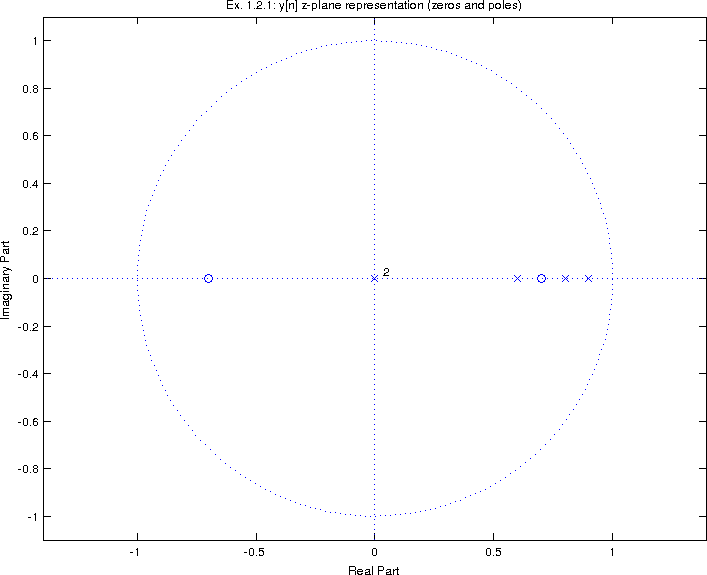
\includegraphics[width=0.65\textwidth]{images/ex1_2_1.png}
	\captionof{figure}{$y[n]$ z-plane representation (zeros and poles).}
	\label{fig:ex1_2_1_zplane}
\end{center}

\noindent Como se pode observar, todos os pólos e raízes estão contidos no círculo de raio unitário. Como tal, este sistema é \textbf{estável}.

\subsubsection{Exercise 1.2.3}
\label{subsubsec:ex1_2_3}
\noindent Dado que assumimos que
\begin{equation}
	G(z) = H(z)|_{\text{condições iniciais nulas}} \\
\end{equation}

\noindent é possível obter a expressão da resposta a impulso do sistema, $h[n]$, válida para $n \ge 0$, aplicando à função de transferência anteriormente obtida a Transformada Inversa de $Z$ ($\mathcal{Z}^{-1}$). Utilizando a função \texttt{iztrans} do \texttt{MATLAB} obteve-se a expressão
\begin{equation}
	h[n] = \mathcal{Z}^{-1}\{G(z)\} = \frac{44573}{31104} \, \delta[n - 1] + \frac{1537}{4320} \, \delta[n - 2] - \frac{1274 \, (\frac{3}{5}) ^ n}{405} - \frac{11767 \, (\frac{4}{5}) ^ n}{2560} + \frac{100397 \, (\frac{9}{10}) ^ n}{21870} + \frac{17644573}{5598720} \, \delta[n]
\end{equation}

\subsubsection{Exercise 1.2.4}
\noindent Em seguida apresenta-se a resposta a impulso do sistema, segundo a expressão obtida em \emph{\nameref{subsubsec:ex1_2_3}} (azul) e segundo as funções do \texttt{MATLAB} \texttt{impz} (vermelho) e \texttt{dimpulse} (verde).

\begin{center}
	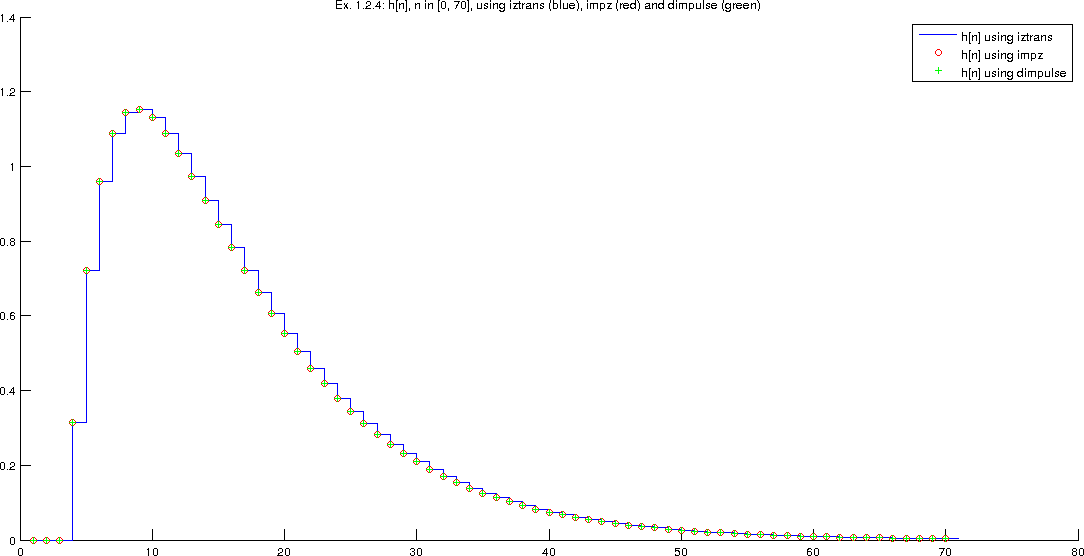
\includegraphics[width=0.70\textwidth]{images/ex1_2_4.png}
	\captionof{figure}{$h[n]$, $n \in [0, 70]$, using \texttt{iztrans} (blue), \texttt{impz} (red) and \texttt{dimpulse} (green).}
	\label{fig:ex1_2_4_zplane}
\end{center}

\subsubsection{Exercise 1.2.5}
\label{subsubsec:ex_1_2_5}
\noindent Considerando que é conhecida a expressão de $H(z)$, é possível obter a resposta do sistema ao degrau unitário ($u[n]$) usando a igualdade
\begin{equation}
	Y(z) = X(z) \, H(z)
\end{equation}

\noindent onde $X(z)$ deverá ser substituída por $U(z)$, Transformada de $Z$ de $u[n]$. $U(z)$ é dada por
\begin{equation}
	U(z) = \frac{1}{1 - z^{-1}}
\end{equation}

\noindent O resultado desse produto dará a Transformada de $Z$ da resposta do sistema ao degrau unitário. Isto é,
\begin{eqnarray}
	Y(z) & = & U(z) \, H(z) \\
	& = & \frac{1}{1 - z^{-1}} \, \frac{0.3137 \, z^{2} - 0.1537}{z^{5} - 2.3 \, z^{4} + 1.74 \, z^{3} - 0.432 \, z^{2}}
\end{eqnarray}

\noindent Como queremos a expressão da resposta do sistema, tem de ser aplicada a Transformada Inversa de $Z$, $\mathcal{Z}^{-1}$. Utilizando a função \texttt{iztrans} do \texttt{MATLAB}:
\begin{equation}
	\label{eq:ex_1_2_5_unit_step_response}
	y[n] = \mathcal{Z}^{-1}\{Y(z)\} = \frac{637 \, \left(\frac{3}{5}\right)^n}{135} - \frac{1537 \, \delta[n - 1]}{4320} + \frac{11767 \, \left(\frac{4}{5}\right)^n}{640} - \frac{100397 \, \left(\frac{9}{10}\right)^n}{2430} - \frac{278197 \, \delta[n]}{155520} + 20
\end{equation}

\subsubsection{Exercise 1.2.6}
\noindent Em seguida apresenta-se a resposta do sistema ao degrau unitário, segundo a equação (\ref{eq:ex_1_2_5_unit_step_response}) (azul) e segundo a função do \texttt{MATLAB} \texttt{dstep} (vermelho).
\begin{center}
	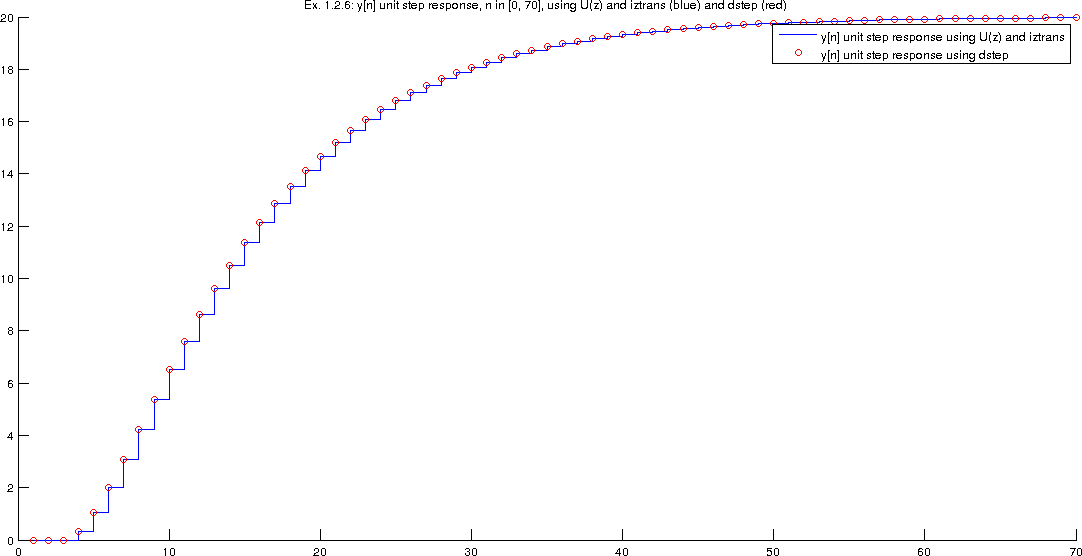
\includegraphics[width=0.70\textwidth]{images/ex1_2_6.png}
	\captionof{figure}{$y[n]$ unit step response, $n \in [0, 70]$, using $U(z)$ and \texttt{iztrans} (blue) and \texttt{dstep} (red).}
	\label{fig:ex1_2_6}
\end{center}

\subsubsection{Exercise 1.2.7}
\noindent Para computar a resposta do sistema para uma dada entrada, considera-se que é dada segundo o formato simbólico do \texttt{MATLAB}. Calcula-se a sua Transformada de $Z$, que por convolução com a função de transferência, origina a Transformada de $Z$ dessa resposta. Após isso, em semelhança a \nameref{subsubsec:ex_1_2_5}, é aplicada a Transformada Inversa de $Z$ ao resultado, o que origina a expressão da resposta do sistema para uma dada entrada. Apresenta-se o resultado para a expressão \begin{center}\texttt{4 * (heaviside(n - 3) - heaviside(n - 9))}\end{center}
\begin{center}
	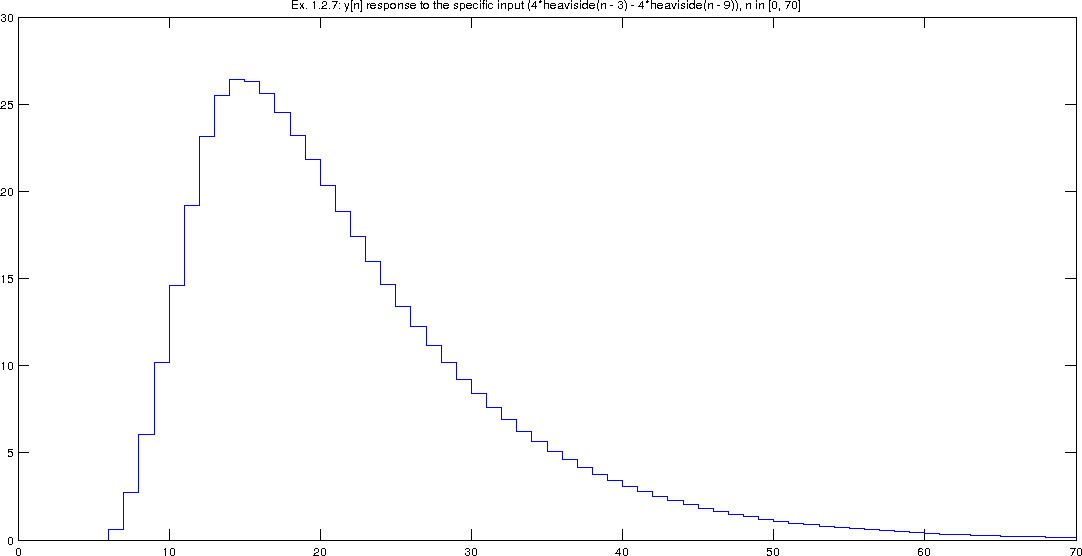
\includegraphics[width=0.70\textwidth]{images/ex1_2_7.png}
	\captionof{figure}{$y[n]$ response to the specific input (\texttt{4 * (heaviside(n - 3) - heaviside(n - 9))}), $n \in [0, 70]$.}
	\label{fig:ex1_2_7}
\end{center}

\end{document}
